%------------------------------------------------------------------------------
% Stijl,Imports en Commando's
%------------------------------------------------------------------------------

%---------- Stijl ----------------------------------------------------
\documentclass{hogent-article}

%---------- Custom Commando's ----------------------------------------------------
\newcommand{\boldit}[1]{\emph{\textbf{#1}}} 
\newcommand{\customref}[1]{\underline{\ref{#1}: \nameref{#1}}}

%---------- Package imports ----------------------------------------------------
\usepackage{lipsum} % Voor vultekst
\graphicspath{{./grafieken/}}
\usepackage{subcaption}
\usepackage{float}

%------------------------------------------------------------------------------
% Metadata over het artikel
%------------------------------------------------------------------------------

%---------- Titel & auteur ----------------------------------------------------

% TODO: geef werktitel van je eigen voorstel op
\PaperTitle{Retrieval practice}
% TODO: geef op welk soort artikel dit is
% Dit is typisch de opdracht en het vak waarvoor dit artikel geschreven is, bv.
% ``Verslag onderzoeksproject Onderzoekstechnieken 2018-2019''
\PaperType{Verslag Onderzoek Onderzoekstechnieken 2018-2019}

% TODO: vul je eigen naam in als auteur, geef ook je emailadres mee!
\Authors{Wannes {De Craene}\textsuperscript{1},Michiel Schoofs\textsuperscript{2}, Lieven {Van Loo}\textsuperscript{3}, Wannes Sergeant\textsuperscript{4}}% Authors

% TODO: vul de naam van je co-promotor in.
% Als het hier gaat om een voorstel voor de bachelorproef, dan ben je hier
% verplicht de naam van je co-promotor in te vullen. Zoniet, dan kan je het
% leeg laten.
% Contactinfo: Geef hier de contactgegevens van elke auteur van het artikel (en
% indien van toepassing ook van de co-promotor).
\affiliation{
	\textsuperscript{1} \href{mailto:wannes.decraene.y0550@student.hogent.be}{mailto:wannes.decraene.y0550@student.hogent.be}
}
\affiliation{
	\textsuperscript{2} \href{mailto:michiel.schoofs@student.hogent.be}{mailto:michiel.schoofs@student.hogent.be}
}
\affiliation{
	\textsuperscript{3} \href{mailto:lieven.vanloo@student.hogent.be}{mailto:lieven.vanloo@student.hogent.be}
}

\CoPromotor{}

%---------- Abstract ----------------------------------------------------------

\Abstract{Veel studenten hebben baat bij een betere studiemethode.De werkdruk in het onderwijs leidt tot stressvolle situaties, een betere methodiek kan helpen om de werkdruk te verlagen en de studenten een hoger slaagpercentage te geven.Doormiddel van dit onderzoek trachten we om een duidelijk overzicht te geven van de zogenaamde \boldit{Retrieval practice} methode.We bekijken de effecten van Retrieval practice voor groepen met een \boldit{Hoge} en \boldit{lage geheugencapaciteit}. Ook proberen we het type van memorisatie doormiddel van deze techniek in kaart te brengen zijnde: \boldit{Rote} of \boldit{Memorisation}.Doormiddel van empirisch onderzoek proberen we eerdere studies te staven en verifiëren. We verwachten dat de conclusies van het eerder onderzoek correct zijn.Dit zou suggereren dat studenten met een lage geheugencapaciteit meer baat hebben bij Retrieval practice.Alsook dat Retrieval practice leidt tot Rote memorisatie en geschikt is voor grote hoeveelheden uit het hoofd te leren maar minder toepaselijk is bij leerstof waar effectief diepgaand begrip van de stof wordt verwacht.
}

%---------- Onderzoeksdomein en sleutelwoorden --------------------------------
% TODO: Vul de sleutelwoorden aan.


\Keywords{Onderzoekstechnieken; Retrieval Practice; Rote; Meaningful; Geheugencapaciteit}
\newcommand{\keywordname}{Sleutelwoorden}

%---------- Titel, inhoud -----------------------------------------------------

\begin{document}

\flushbottom % Makes all text pages the same height
\maketitle % Print the title and abstract box
\tableofcontents % Print the contents section
\thispagestyle{empty} % Removes page numbering from the first page

%------------------------------------------------------------------------------
% Hoofdtekst
%------------------------------------------------------------------------------

\section{Inleiding}

Retrieval practice en het zogenaamde test effect is door verschillende instellingen en experten reeds onderzocht, geprezen en genuanceerd. Zelfs tijdens het schrijven van deze literatuurstudie is er nieuw onderzoek verschenen door \textcite{Moreira_2019}. Door de hoeveelheid van studies en publicaties is het moeilijk om het bos door de bomen te zien. We zullen proberen aan de hand van een aantal onderzoeken een overzicht te geven van wat deze studiemethode inhoud en hoe studenten het best kunnen gebruik maken van deze studietechniek.\\
\par
\noindent
Concreet zullen we drie verschillende onderzoeken samenbrengen tot één experiment:\\
\begin{itemize}

\item Ons eerste doel is de originele studie van \textcite{Roediger_2006}  reproduceren en evalueren. we kuhjen met andere woorden of er inderdaad spraken is van het zogenaamde '\boldit{Test effect}'. - Voor meer informatie zie \customref{RetrievalPractice} -\\

\item Vervolgens willen we eveneens de studie van \textcite{Agarwal_2016} opnemen binnen ons onderzoek. Deze studie suggereert dat mensen met een lagere geheugencapaciteit meer baat hebben bij Retrieval practice. - Zie ook\\ \customref{geheugencapaciteit} -\\

\item Tot slot bestuderen we nog het type van memorisatie dat bereikt wordt doormiddel van Retrieval practice. Concreet onderscheiden we twee types van memorisatie namelijk: ROTE en meaningful learning. Zoals het onderzoek van \textcite{van_Gog_2012} suggereert verwachten we dat de studenten de informatie van buiten leren (ROTE) zonder deze effectief te begrijpen (Memorisation). -Zie ook \customref{RoteVSMeaningful} -
\end{itemize}

\section{Overzicht literatuur}

Voor we kunnen van start gaan met het onderzoek moeten we eerst een literatuurstudie schrijven om duidelijk uit te lijnen welke bevindingen er reeds zijn binnen dit vakgebied. Deze sectie dient eveneens voor het verduidelijken van de terminologie dat we gebruiken binnen ons experiment. Na het lezen van deze literatuurstudie hopen we dat de relevantie van de door onze gekozen variabelen duidelijk zijn.

\subsection{Retrieval Practice}
\label{RetrievalPractice}
Wat verstaan we nu juist onder de term `Retrieval Practice`? Concreet is dit een systeem waarbij je leerstof gaat leren door het afnemen van testen, in de plaats van gewoon een boek te nemen en het op conventionele wijze te gaan studeren.\\
\par
\noindent
Om dit te verduidelijken halen we de methodiek aan zoals beschreven in het artikel van \textcite{Roediger_2006}. Een groep van testpersonen werd gevraagd om een nooit eerder geziene tekst van buiten te leren volgens verschillende methoden.\\\\De eerste groep werd gevraagd om de tekst te bestuderen gedurende 20 minuten op de manier waarop ze het meest vertrouwd waren. De andere groep kreeg slechts 5 minuten om de tekst te bestuderen en werd vervolgens gevraagd om gedurende 15 minuten de tekst te reproduceren op papier (het reproduceren op papier noemen we ook testen).\\

\par
\noindent
De laatste methodiek namelijk het bestuderen en vervolgens reproduceren op papier duiden we aan als \boldit{Retrieval practice}. Uit de originele studie van Roediger en Karpicke bleek dat de groep die aan Retrieval practice deed veel meer van de originele tekst onthield na twee weken dan de groep die conventioneel studeerde. Dit fenomeen bestempelt men ook als het `\boldit{Testing effect}`.

\subsection{Onderscheid in geheugen capaciteit}
\label{geheugencapaciteit}
De studie van \textcite{Agarwal_2016} stelt dat er een onderscheid is tussen personen met een Lage en Hoge geheugencapaciteit. De bevindingen van het onderzoek wijzen uit dat Retrieval practice veel meer resultaat biedt bij proefpersonen met een lagere geheugencapaciteit. \textcite{Agarwal_2016} beweert zelfs dat Retrieval practice een effectieve leer strategie kan zijn voor lager presterende studenten.\\
\par
\noindent
We zullen deze studie reproduceren, doormiddel van onze testgroep onder te verdelen in twee groepen. Voor een meer gedetaileerde uitleg zie\\ \customref{methodologie} .

\subsection{Wat is leren?}
Wat wordt er nu exact verstaan onder de term '\textit{leren}'? Het artikel van \textcite{Mayer_2002} zegt dat leren niet enkel het verkrijgen van informatie is, maar dat men ook rekening moet houden met het toepassen van deze informatie op nieuwe en relevante stuaties. Concreet definieert men in het artikel het leerproces in termen van twee fasen namelijk:\\

\begin{itemize}
	\item \textbf{Het behouden van informatie}: hierbij zal de student de informatie bewaren over een lange periode van tijd. We spreken hier dus over het vermogen van de persoon tot het onthouden van informatie en deze te kunnen ophalen in haar originele vorm. We hebben het hier dus \underline{niet} over interpreteren van informatie maar puur over het memoriseren in haar originele vorm.\\
	
	\item \textbf{Toepassen van informatie}: Hiermee bedoeld men het vermogen om de nieuw opgedane kennis toe te passen. Het  gaat hier dus niet alleen over het ophalen van informatie maar eveneens het interpreteren en toepassen. Deze fase is dus een vervolg op de vorige fase en kan niet als losstaand aanzien worden.
\end{itemize}

\subsection{Rote vs Meaningful Learning}
\label{RoteVSMeaningful}
Het artikel van \textcite{Mayer_2002} bestempelde deze twee fasen eveneens als: Rote (Behouden van informatie) en Meaningful learning(Toepassen van informatie). Uit een vervolg studie door \textcite{van_Gog_2012} blijkt dat Retrieval practice voornamelijk tot Rote memorisatie leidt.\\

\par
\noindent
Met andere woorden is de proefpersoon doormiddel van deze techniek beter instaat de informatie op te halen in zijn originele vorm. Indien men echter gaat kijken naar het vermogen van de persoon om deze informatie te verwerken in concrete problemen (\textit{Meaningful learning}) ziet men het omgekeerde effect. Men stelt in het onderzoek dat Retrieval practice zelfs nadelig is op Meaningful learning en dat conventioneel studeren een betere optie is voor het verwerken van informatie.\\
\par
\noindent

\subsection{Retentie testen}
Een ander begrip binnen Retrieval practice is dat van de zogenaamde \boldit{retentie testen}. Een retentie test is de methode waarmee men gaat meten hoeveel informatie effectief onthouden is en wordt gebruikt om de noodzakelijke data voor de conclusies te verzamelen. In het originele experiment \textcite{Roediger_2006} werd gebruik gemaakt van een vragenlijst over de tekst.\\

\par
\noindent
Deze methodiek kunnen we echter niet gebruiken indien we spreken over Meaningful learning.Omdat deze manier van testen voornamelijk dient voor het meten van het behoud van informatie (Rote). Als reactie hierop ontwikkelde \textcite{Mayer_2002} een andere vorm van retentie test. De opzet van deze ontwikkeling was om te bepalen hoe effectief de proefpersonen de aangereikte informatie hadden verwerkt.\\
\par
\noindent
Om de methode van Mayer het best weer te geven maken we gebruik van zijn analogie. Hij stelde dat de gebruikte tekst over de wet van ohm (een wet uit de natuurkunde) ging en de koppeling van deze wet op elektrische circuits. Klassiek zou men vervolgens een vragenlijst geven over deze wet en de geziene informatie. De methode die hij echter voorstelde was een reeks oefeningen op deze wet te geven alsook een vraagstuk waarin men deze wet moest toepassen op een circuit en de resistentie bepalen. - Dit is ook de exacte methodiek die gebruikt werd in het onderzoek van \textcite{van_Gog_2012} om de mate van Meaningful learning te bepalen. -

\subsection{Invloed Feedback op Retrieval Practice}

Een belangerijke factor binnen het originele onderzoek van \textcite{Roediger_2006} was dat de zelftesten (na de originele studie van de tekst) zonder enige feedback waren. Dat wou zeggen dat indien de proefpersoon foutieve informatie opschreef op de zelftest deze informatie ook foutief werd opgenomen in het geheugen.\\
\par
\noindent
In het onderzoek van \textcite{Roediger_2011} leerde we dat feedback door externe zeker niet te verwaarlozen is. Het verschil tussen wel en geen feedback is aanzienlijk: in het geval van hun onderzoek waren de resultaten van de groep met feedback 30\% tot 64\% beter dan de testgroep zonder feedback.

\subsection{Invloed van voorkennis van de stof op de prestaties geleverd door Retrieval practice}

Een laatste stelling die we nog zouden willen meegeven is dat de mate van voorkennis, geen invloed heeft op de resultaten geboekt doormiddel van Retrieval practice.\\
\par
\noindent
Deze stelling werd op de proef gesteld door het onderzoek van \textcite{Xiaofeng_2016}. In deze studie onderzocht men het effect van voorkennis op twee verschillende studiemethodes namelijk Elaboration en Retrieval practice. Elaboration is een techniek waar er gebruik gemaakt wordt van relaties tussen reeds bestaande kennis en nieuwe kennis om op die manier efficiënter te gaan leren. Uit dit onderzoek bleek dat bij Retrieval practice de mate van voorkennis weinig tot geen invloed had op de retention tests; en dit in tegenstelling tot Elaboration.\\
\par
\noindent
In andere woorden studenten die reeds vertrouwd waren met het onderwerp van de gegeven tekst hadden geen voordeel ten opzichte van de groep die minder vertrouwd was met het onderwerp.

\section{Methodologie}
\label{methodologie}
Om bovenstaande variabelen te kunnen gebruiken in onze conclusies moeten we ook uitlijnen hoe we deze willen gaan testen. Onder deze sectie vindt u een voorstel over hoe we deze verschillende variabelen op een empirische manier zouden kunnen meten.

\subsection{Meten van geheugencapaciteit}
\label{methodology-gc}
Naar aanleiding van het artikel van \cite{Agarwal2016} gaan we onderzoeken of er een correlatie is tussen de geheugencapaciteit en de doeltreffendheid van Retrieval Practice. -Voor meer informatie zie ook sectie \customref{geheugencapaciteit}.- We moeten echter eerst verduidelijken hoe we deze capaciteit zouden gaan meten in onze testgroepen.\\
\par
\noindent
We kunnnen gebruik maken van een woordenlijst van 25 woorden elk toenemend in lengte. De proefpersoon in kwestie krijgt 5 minuten om de woordenlijst te memoriseren en wordt vervolgens gevraagd om deze te reproduceren. Daarna wordt een score toegekend volgens volgend principe: Een volledig correct geschreven woord krijgt 2 punten, een woord dat fonetisch correct is krijgt 1 punt.\\
\par
\noindent
Door deze methode te hanteren zijn we instaat om de groep in twee delen op te splitsen. De groep die hoger scoorde dan de mediaan bestempelen we als \textit{Hoge geheugencapaciteit} de overige groep benoemen we als \textit{Lage geheugencapaciteit}

\subsection{Hervorming van de retentie test}
We gaan eveneens de retentie test veranderen. Dit doen we naar aanleiding van het artikel geschreven door \cite{TamaravanGog2012}. Concreet willen we het type van memorisatie (ROTE of Meaningful) door Retrieval Practice gaan bestuderen. -Voor meer informatie zie sectie \customref{RoteVSMeaningful}.-

\section{Verwachte resultaten}
\subsection{Hypothesen}
\subsection{Duiding}

Analoog aan de artikels van \cite{HenryRoediger2006} en \cite{Agarwal2008}, zullen we gebruik maken van zowel grafieken als tabellen om onze hypotheses te staven. Op deze manier kunnen we de gebruikte dataset vereenvoudigen en op een compacte en correcte manier conclusies gaan trekken.\\
\par
\noindent
We zouden graag toch een moment nemen om stil te staan bij de verschillende variabelen en veronderstellingen die we gebruiken om deze grafieken te maken. Zo hopen we foutieve communicatie te voorkomen.

\subsection{Grafieken}
\subsubsection{Uitleg}
De grafieken die we gebruiken zijn opgedeeld in twee groepen (uitgeleind in sectie \customref{methodology-gc}):
\begin{itemize}
	\item De groep met een \textit{lage geheugencapaciteit (LGC)}: Dit is de testgroep die op de voorafgenomen woordenlijst onder de mediaan scoorde. Deze testgroep zit dus met andere woorden in de laagste 50\% van de afgenomen testen betreffende hun score.
	\item De groep met een \textit{hoge geheugencapaciteit (HGC)}: Dit is de groep die boven de mediaan scoorde. Kortom de groep die bij de hoogste 50\% zit qua hun score op de woordenlijst.
\end{itemize}


\subsubsection{Grafieken}
\begin{figure}[H]
	\begin{subfigure}{0.45\textwidth}
		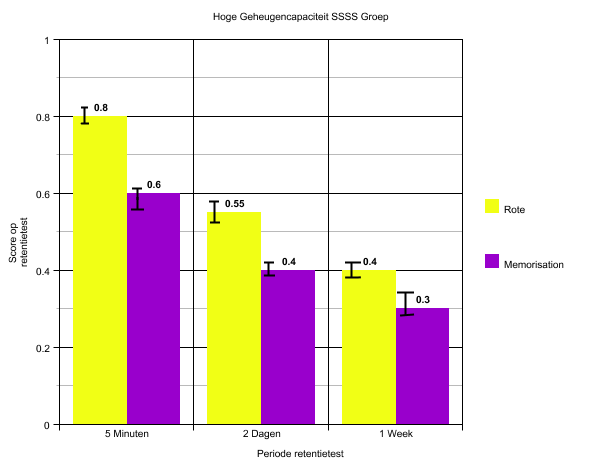
\includegraphics[width=\linewidth]{grafiek1}
		\caption{HGC Grafiek SSSS}
	\end{subfigure}
	\begin{subfigure}{0.45\textwidth}
		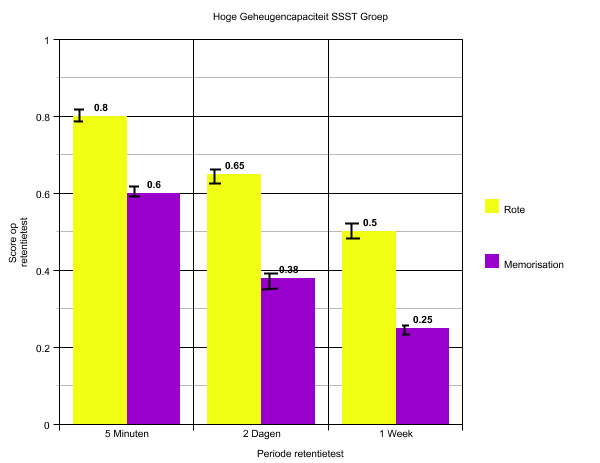
\includegraphics[width=\linewidth]{grafiek3}
		\caption{HGC Grafiek SSST}
	\end{subfigure}
	\begin{subfigure}{0.4\textwidth}
		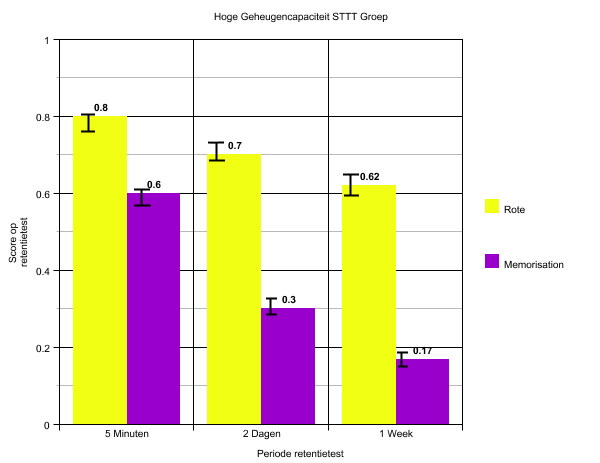
\includegraphics[width=\linewidth]{grafiek5}
		\caption{HGC Grafiek STTT}
	\end{subfigure}
	\caption{Grafieken van de Hoge Geheugencapaciteit groep}
\end{figure}

\section{Conclusie}

\subsection{Variabelen}
Concreet hebben wij beslist om een extra variabele te gaan introduceren, namelijk de geheugencapaciteit van het proefpubliek. Ook hebben wij beslist om de retentietest te hervormen volgens twee principes: Rote en Meaningful Learning (lees als uit het hoofd leren en kunnen toepassen).\\
\par
\noindent    
Verder delen we de proefpersonen op in drie groepen, idem aan het originele experiment door \cite{Henry2006} , Deze zijn: Study-Study-Study-Study, Study-Study-Study-Test  en Study-Test-Test-Test. 

\subsection{Hypothesen en resultaten}

\noindent
Eerst en vooral verwachten we dus als conclusies een gelijkaardig resultaat dan het vooraf afgenomen onderzoek van \cite{Henry2006}. Dit wil zeggen dat mensen die aan retrieval practice doen beter zouden moeten scoren dan mensen die op conventionele wijze studeren.\\
\par
\noindent
Bovenop voorgaand resultaat verwachten we ook dat mensen met een lage geheugencapaciteit iets meer hulp zullen zien indien ze gebruik maken van Retrieval Practice.\\
\par
\noindent
En als laatste verwachten we een beter resultaat bij de groepen studenten die aan Rote learning doen, in vergelijking met student die aan Meaningful learning doen.


\section{Addendum}

Verder hebben we nog enkele artikels die zeer nuttige info bevatten, maar die niet absoluut noodzakelijk zijn voor het succesvol af te werken van het experiment, daarom hebben wij deze dus ter info nog toegevoegd.

\subsubsection{Successful inhibition, unsuccessful retrieval: Manipulating time and success during retrieval practice}

Hier spreekt men eigenlijk over exact hetzelfde als ons, maar op een omgekeerde wijze. Wat bedoelen we hier juist mee? Wel, in het vooraf uitgevoerde experiment van \cite{HenryRoediger2006} teste men op het behouden van informatie, in dit artikel van \cite{BenjaminStorm2009} bekeek men wat de proefpersonen vergaten. Dit is dus niet echt noodzakelijk artikel, maar het blijkt wel interessant om te zien dat het omgekeerde experiment tot een quasi idem resultaat leid. Dit artikel werd geschreven door. 

\subsubsection{Commentary: Retrieval practice protects memory against acute stress}

In dit artikel van \cite{Smith2016} bekijkt men welke invloed ``Retrieval Practice'' heeft op stress, terwijl dit wel een goede variabele zou zijn om op te nemen in dergelijke onderzoeken hebben wij beslist om onze focus ergens anders te leggen.

\subsubsection{Optimizing retrieval as a learning event: When and why expanding retrieval practice enhances long-term retention}

Dit artikel, geschreven door \cite{Storm2010} is zo goed als een ``kopie'' van het voorafgenoemde artikel van \cite{HenryRoediger2006}, dit kunnen we dus ook niet echt opnemen in onze studie, maar het is handig om te zien dat er een volledig losstaand onderzoek tot een zeer gelijkaardig resultaat komt. 

\subsubsection{Retrieval Practice Produces More Learning than Elaborative Studying with Concept Mapping}

Aangezien men spreekt over een nieuwe studiemethode was het ook interessant om te bekijken of er nu nog andere methodes dan enkel Retrieval Practice zijn die bevorderend werken voor de retentie van geziene leerstof. \cite{JeffreyKarpicke2011} voegt hier een extra studiemethode genaamd ``Concept Mapping'' uit, dit had dus ook een leuke variabele kunnen zijn voor ons onderzoek, maar zoals voordien vermeld zijn wij een andere weg op gegaan.

%------------------------------------------------------------------------------
% Referentielijst
%------------------------------------------------------------------------------

\phantomsection
\printbibliography[heading=bibintoc]

\end{document}
